\section{Pojačano učenje}
Najistaknutije osobine pojačanog učenja su pokušaj i neuspjeh, te odgođena nagrada koje algoritam doživljava u okruženju. Algoritam bi trebao, do neke razine, imati osjećaj i informacije o okolini, te cilj ili cilevi prema kojima teži, a odnose se na određeno stanje u okolini.

\subsection{Umjetna inteligencija}
Je jako široko područje računalne znanosti. Bavi se proučavanjem i izrade algoritama koje nemaju explicitnih naredbi kako se ponašati u nekom trenutku i/ili okolini, nego kroz određene procese sami uspiju donijeti zaključke i odluke. Umjetna inteligencija se dijeli u puno pod grana, koje u prošlosti nisu uspješno međusobno surađivali. U današnje doba se iskazao potencijal umjetne inteligencije i sve više se ulaže u njezino istraživanje i razvoj. 

Umjetna inteligencija se djeli na više grana kao što su:
\begin{itemize}
	\item Rasuđivanje i rješavanje problema: Gdje se pokušava implementirati razbivanje problema u logičke korake do riješenja te postepenim izvršavanje koraka riješiti zadani problem. Ovakvi algoritmi se nisu iskazali korisnim u velikim problemima zbog kombinatorijske eksplozije, znači rastom problema algoritam exponencijalno usporava.
	
	\item Reprezentacija znanja: Ovo je glavno područje u istraživanju klasične umjetne inteligencije. Skuplja se znanja od nekog područja i pohranjuje se u neku bazu u kojoj se istaknu pojmovi i veze između njih. Neke od stvari koje bi se nalazili u takvoj bazi su: predmeti, svojstva, vrste i odnose između predmeta, situacija, događaje, stanja i vremena, uzroci i posljedice, znanje o znanje i još puno manje istraženih područja.
	
	\item Planiranje: Odnosi se na predviđanje nekih budućih događaja te donošivanje određenih odluka koje utječu na izhod.
	
	\item Učenje: Predstavlja algoritme koji is početka jako loše riješavaju zadatak, međutim skupljanjem iskustva vremenom su sve bolje.
	
	\item Obrada prirodnog jezika: Omogućuje strojevima razumjevanje ljudskih jezika.
	
	\item Percepcija: Sposobnost pomoću određenih senzora primit informacije o stvarnoj okolini te uspješno interpretiranje te informacije u svoje zadaće.
	
	\item Kretanje i rukovanje: Upravljanje mehaničkih udova kako bi riješilo neki zadatak u stvarnoj okolini. Smatra se posebno kompleksnim, te obuhvaća paradoksni pojam (Moravec's paradox) u kojemu je teže implementirati radnju koju mlado dijete može izvoditi bez ikakvih poteškoća kao npr: primit neki predmet u ruke i odložit ga na odrećeni položaj od radnje kojoj je odraslome čovjeku teško kao npr: jako dobro odigrati partiju šaha. Prizlazi iz činjenice da za razliku od šaha percepcija, kretanje i rukovanje su prirodnom selekcijom kroz miljunima godinama usađeni u čovjeka.
	
	\item Socijalna inteligencija: Uključuje poznavanje i prepoznavanje emocije i ljudskih međudjelovanja. Nekim algoritmima bi bilo vrlo korisno da uz pojmove teorije uključuje spoznaju ljudskih emotivnih stanja i motive za donijeti bolje odluke.
	
	\item Opća inteligencija: U prošlosti se pokušalo dizajnirati opće inteligentnog agenta koji pokriva široku ljudsku spoznaju. No odustalo se od toga, zbog preogromne količine inforamcije koja je kombinirana iz raznih područja. Danas se razvija 'usku' umjetnu inteligenciju koja je usredotočena u jedno područje i smatra se da opća umjetna inteligencija bi trebala ujedinit hrpu tih usredotočenih područja.
\end{itemize}

\subsection{Strojno učenje}
U ovome završnom radu se razradilo područje iz učenja. Pa tako i ovo područje se grana na više podpodručja. Među najpoznatijima su učenje sa nazorom (eng. \textit{supervised learning}) u kojemu algoritam dobije skup podataka iz kojih treba donijet neke zaključe te skup riješenja, odnosno definirane zaključke koje bi trebao donijeti. Tako da kroz nekog vremena koje je dodjeljeno za učenje, primi podatak, donese odluku i ovisno 
o tome koji je unaprijed definirani zaključak kojeg je trebao donijeti se prilagodi da u buduće donosi što ispravnije odluke. Druga grana se zove učenje bez nazora (eng. \textit{unsupervised learning}), gdje algoritam prima neki skup podataka i vremenom uspije pronaći razlike i sličnosti u podacima. Nema informacije o tome šta podatak predstavlja ali zna podatke svrstiti u svoje definirane kategorije. Izrađeni agent iz ovog projekta spada pod skupinom pojačano učenje (eng. \textit{reinforcement learning}). U ovoj grani algoritam djeluje u nekom okruženju pomoću određenih akcija, te u početku nema informacije o tome kako akcije utječu na okruženje. Te vremenom mora sam otkriti koje akcije u kojem trenutku donosi najveću nagradu.


\subsection{Povijest pojačanog učenja}
---> POVJEST ODE <---

\subsection{Elementi pojačanog učenja}
Osnovni građevni blokovi na kojem se temelju metode pojačanog učenja su:
\begin{itemize}
	\item Politika: Opisuje ponašanje u određenom trenutku. Određuje koje radje poduzeti ovisno o stanju okruženja, iskazuje se kao funkcija vjerojatnosti koja opisuje vjerojatnost sljedeće određene radnje.
	
	\item Signal nagrade: Govori algoritmu koliko je uspješan i primarni cilj svakog algoritma pojačanog učenja je težiti prema najvećoj mogućoj nagradi. 
	
	\item Funkcija vrijednosti: Daje određenoj situaciji konkretnu vrijednost. Na neki način procjenjuje buduću nagradu, što ga čini sekundarnim ciljem algoritmu pojačanog učenja. Uspješnim predviđanjem dugoročne nagrade poboljšava i ubrzava process izvršavanje primarnog cilja. 
	
	\item Model okruženja: Neobavezni element, koji oponaša okruženje. Pomaže algoritmu planirati buduća ponašanja. Algoritmi koji se služe modelom nazivaju se metode bazirane na modelu (eng. \textit{Model based}) za razliku jednostavnijim metodama slobodni od modela (eng. \textit{Model free}).
\end{itemize}

\subsection{Konačan Markov proces odlučivanja}
Formalizacija sekvencijalnog postupka donošenje odluka u kojima se uključuje, osim neposredne nagrade, odgođena nagrada. Procjenjuje se vrijednost za svaku radnju u nekom stanju $q_*(s,a)$ ili vrijednost stanja $v_*(s)$. 

Osnovni elementi su:
\begin{itemize}
	\item Agent
	\item Okruženje
	\item Stanje
	\item Akcija
	\item Nagrada
\end{itemize}

Svaka okolina se sastoji od skup stanja $S$ te definira dozvoljene akcije $A$. Osim toga još mora na neki način opisati nagrade $R$. Skupovi $S$, $A$ i $R$ se smatraju konačnim, te za svaki korak $t=0,1,2,...$ u okruženju, agent doživljava stanje $S_t \in S$ i bira akciju $A_t \in A$.


U markovom procesu odlučivanja (eng. \textit{Markov decision process}) se definiraju skupovi za stanja $S$, akcije $A$ te nagrade $R$. Svi skupovi se smatraju konačnim, te u svakom vremenskom koraku $t = 0, 1, 2, ..$, agent proučava stanje $S_t \in S$. U svakom vremenskom koraku pridružena akcija stanju daje par $(S_t, A_t)$, te izvršavanje agentovu radnju okruženje prelazi u sljedeće stanje $S_t+1 \in S$. U novom stanju agent primi nagradu $R_t+1 \in R$ i proučava novo stanje kako bi primjenio sljedeću akciju. Ovaj proces se može opisati funkcijom $f(S_t, A_t) = R_t+1$, te interakcija agenta i okruženja prikazana je na slici~\ref{fig:mdp_diagram}.
\\[\intextsep]
\begin{minipage}{\linewidth}
	\centering%
	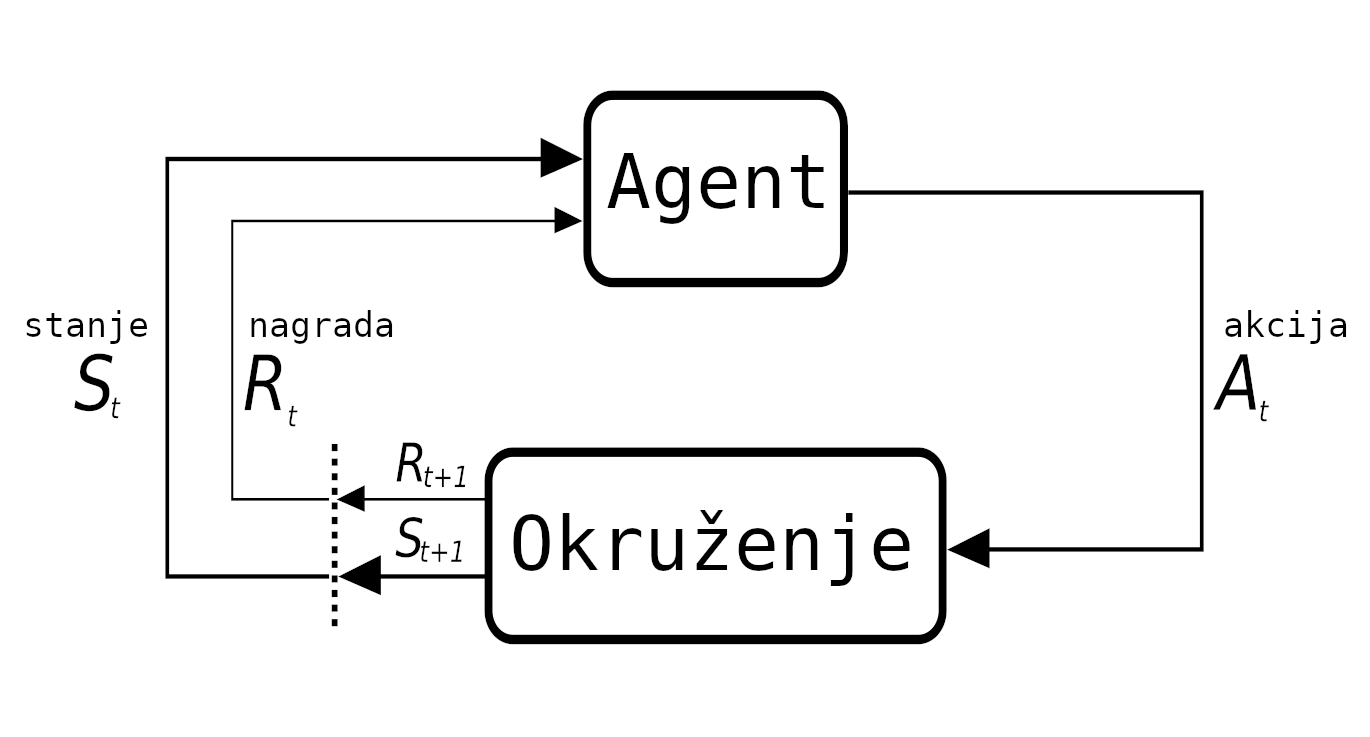
\includegraphics[width=0.8\linewidth,clip=]{images/mdp_diagram.png}%
	\figcaption{Diagram markovog procesa odlučivanja}%
	\label{fig:mdp_diagram}%
\end{minipage}
\\[\intextsep]

\subsection{Nagrada}
Očekivana nagrada $G_t$ se računa kao zbroj svih budućih nagrada $G_T = R_{t+1}+R_{t+2}+R_{t+3}+ ... + R_T$, gdje $R_T$ predstavlja nagradu u konačnom stanju okruženja. Prolaženjem jednom od početnog stanja do krajnog naziva se \emph{epizoda}, tako da pokretanje nove epizode okruženje se ponovno namjesti na neko određeno stanje neovisno o tome kako je prijašna epizoda završila. Međutim kako je agentu važnija neposredna nagrada, a osim toga postoje okruženja u kojima se neprekidno prelazi iz stanja u stanja i okruženje ne posjeduje konačno stanje, uvodi se pojam \emph{popust budućih nagrada}. Tako da za svaku sljedeću buduću nagradu uzme sve manje u obzir. Ovakva očekivana nagrada se definira kao $R_{t+1} + \gamma R_{t+2} + \gamma ^2 R_{t+3}+...$, gdje gamma predstavlja stopu popusta budućih nagrada, $0 \leq \gamma \leq 1$, tako da sada $G_T$ opisan jednadžbom~\ref{eq:suma_budućih_nagrada_s_popustom}.
\begin{equation}\label{eq:suma_budućih_nagrada_s_popustom}
	G_T = \sum_{k=0}^{\infty} \gamma^k R_{t+k+1}
\end{equation}

\subsection{Politike i funkcije vrijednosti}
Politika određuje agentov sljedeći potez, kroz skupljanje iskustva ta politika se može mijenjati. Označava se sa $\pi$ i definira distribuciju vjerojatnosti preko $a \in A(s)$ za svaki $s \in S$, tako da konačne vjerojatnosti svake akcije $a = A_t$ u stanju $s = S_t$ opisane su policom $\pi(a|s)$.
Za opisivanje agentu dali se nalazi u dobrom stanju ili opisivanje agentu koliko je dobra akcija za neko stanje zadužene su funkcije vrijednosti. Koliko je dobro stanje, odnosno koliko je dobra neka akciju u nekom stanju agentu se daje do znanja pomoću vrijednosti očekivane nagrade. Funkcije vrijednosti se definiraju u odnosu na policu, pošto ona utječe na donošivanje agentove odluke.
Jedna od funkcije vrijednosti je funkcija vrijednosti stanja i pomoću nje agent dobije informaciju o očekivane nagrade, dok prati policu $\pi$, počevši od stanja $s$ u trenutku $t$. Formalno se označava matematičkom jednadžbom~\ref{eq:state_value_function}.
\begin{equation}\label{eq:state_value_function}
	\begin{split}
		v_\pi(s) &= \mathbb{E}_\pi[G_t | S_t = s] \\
				 &= \mathbb{E}_\pi\left[\sum_{k=0}^{\infty} \gamma^k R_{t+k+1} | S_t = s\right]
     \end{split}
\end{equation}
S druge strane postoji funkcija vrijednosti akcija $q_\pi(s, a))$ koja opisuje koliko je dobra akcija $a$ u stanju $s$ dok se prati politika $\pi$. Tako da funkcija računa vrijednost očekivane nagrade za svaku akciju i definirana je matematičkom jednadžbom~\ref{eq:action_value_function}.
\begin{equation}\label{eq:action_value_function}
\begin{split}
q_\pi(s, a) &= \mathbb{E}_\pi[G_t | S_t = s, A_t = a] \\
&= \mathbb{E}_\pi\left[\sum_{k=0}^{\infty} \gamma^k R_{t+k+1} | S_t = s, A_t = a\right]
\end{split}
\end{equation}
Slovo $q$ opisuje kvalitetu (eng. \textit{quality}) određene akcije i često se vrijednost naziva q-vrijednost, te funkcija koja je daje q-funkcijom. U jednadžbama~\ref{eq:state_value_function} i ~\ref{eq:action_value_function} $\mathbb{E}_\pi$ definira očekivanu vrijednost, u ovom slučaju očekivanu nagradu, slučajne variable praćenjem politike $\pi$.

\subsubsection{Optimalne politike i funkcije vrijednosti}
Jedna od osnovnih značakih pojačanom učenju koja se ističe, je da algoritam ima neki definirani cilj, prema kojemu teži. Glavni cilj je pronalaženje optimalne politike, koju će agent pratit, kako bi doveo nagradu do najveće moguće razine. Neka politika $\pi$ se smatra boljom od neke druge politike $\pi'$, ili bar jednako dobro, ako za sva moguća stanja nudi višu, ili jednaku nagradu za agenta. Optimalna politika je je ona koja za sva moguća stanja daje najveću nagradu i kada ne postoju neka druga politika koja za neko stanje daje veću nagradu. Također optimalna politika posjeduje njoj pripadajuću optimalnu funkciju vrijednosti stanja, odnosno optimalnu funkciju vrijednosti akcija. Optimalne funkcije se bilježe $v_*$ gdje $v_*(s) = \max_\pi v_\pi(s)$ za funkciju vrijednosti stanja, a za funkcije vrijednosti akcija $q_*$ gdje $q_*(s, a) = \max_\pi q_\pi(s, a)$ i to za sva $s \in S$, te u slučaju funkcije vrijednosti akcija još i za sva $a \in A$.

\subsection{Bellmanova jednadžba optimalnosti}
U nastavnom djelu ovoga rada usredočenje će biti na $q_*$, tako da se $v_*$ neće razrađivati. To ne znači da to nije primjenivo za $v_*$, ali izrada agenta ide u smjeru q-učenje (eng. \textit{q-learning}), pa je sav daljan opis prilagođen za to. 
Po Bellmanovoj jednadžbi, koju bi trebao svaki algoritam kojemu je cilj pronalaženje optimalne funkcije vrijednosti zadovoljiti, svaka očekivana nagrada jednaka je trenutačnoj nagradi dodana na maksimalne buduće nagrade sa popustom. Ima za zadatak pronaći $q_*$ koja zadovoljava jednadžbu~\ref{eq:bellman_optimality_equation}.
\begin{equation}\label{eq:bellman_optimality_equation}
q_*(s, a) = \mathbb{E}\left[R_{t+1} + \gamma\max_{a'}q_*(s', a')\right]
\end{equation}
Trenutačno stanje i akcija predstavljeni su sa $s$ i $a$, iz koji proizlazi nagrada $R_{t+1}$. Pa je toj nagradi za bilo koje buduće stanje $s'$ i buduće akcije $a'$ dodana vrijednost maksimalne buduće nagrade sa popustom. Pošto se donosi optimalnu akciju u stanju $s$, očekuje se da će se u sljedećemu stanju $s'$ moći izvršiti optimalnu akciju $a'$.

\subsection{Q-Učenje}
Ideja q-učenju jest tablica u kojoj je svaki redak određeno stanje u okolini, a svaki stupac određena akcija za tu okolini. Tako da u svakoj ćeliji se nalazi q-vrijednost za odeđenog para stanja i akcije. Početne q-vrijednosti postavljene su na nulu, jer agent još nije posjetio niti jedno stanje i nema ikakvih informacija o okolini. Prolaženjem kroz stanja okoline i izvršavanje akcije se te q-vrijednosti ažuriraju, tako da češćem izvršavanjem iste akcije u nekom stanju ta q-vrijednost se sve više približava stvarnoj. Pošto tablica u početku nema korisnih informacija o tome koje akcije poduzeti uvodu se pojmove istraživanja (eng. \textit{exploration}) i iskorištavanje (eng. \textit{exploitation}). Gdje u fazi istraživanja agent donese nasumičnu odluku, tako da u sljedećemu stanju primi nagradu i ovisno o tome može ažurirati q-vrijednost u tablici. Istraživanje služi za prikupljanje informacije o okolini kako bi se u buduće moglo donijeti što bolju odluku. U fazi iskorištavanja agent izvrši po njemu najbolju akciju, odnosno pronađe redak u q-tablici koji odgovara trenutačnom stanju i ovisno o tome koja akcija sadrži najvišu q-vrijednost, ta je akcija izabrana. A ta faza služi za prikupljanje najviše moguće nagrade, što je ipak i agentov glavni zadatak.

\subsubsection{Epsilon pohlepna strategija}
Potreban je neki omjer koji raspoređuje koliko i kada će se istraživati, odnosno iskorištavati. Želi se izbjeći istraživanje kada se posjeduje dovoljno informacija o okolini i izostat maksimalnoj nagradi, a također se želi izbjeći iskorištvati sa nedovoljno informacija o okolini, što isto tako dovodi do neuspješnog prikupljanje maksimalne nagrade. Taj omjer u epsilon pohlepnoj strategiji (eng. \textit{epsilon greedy strategy}) je $\epsilon$ i broj je između 0 i 1. Odluka se donosi na način da se nasumično generira broj između 0 i 1, te ako je taj broj veći od $\epsilon$ onda se iskorištava, znači izabere se akcija koja bi trebala donjeti najvišu nagradu, ako je manji onda se istražuje i izvrši se nasumična akcija. Što dovodi do zaključka da sa $\epsilon = 1$ je 100\% sigurno da će se istraživati a kada je $\epsilon = 0$ se neće nikako. Kako se situacije razlikuju dali agent posjećuje svoje prvo stanje ili je već neko vrijeme proveo u okolini i prošao dosta stanja, se prema tome mora i prilagoditi $\epsilon$. Za prilagođavanje koristi se stopa propadajućeg epsilona (eng. \textit{epsilon decay rate}), tako da na početku je $\epsilon = 1$ i vremenom opada i sve više se približava 0. Znači da je na početku agentu veći prioritet iztraživati okolinu i vremenom sve više i više iskorištava. Po terminologiji algoritama se smatra nekim algoritmom \emph{pohlepnim} kada uzme u obzir samo neposrednu vrijednost, odnosno nagradu, u obzir bez da se razmatra dugoročne posljedice. Pa se zbog toga kaže da agent vremenom postane pohlepan. Najčešće se $\epsilon$ nikad ne dosegne vrijednost nule, nego ga se prestane smanjivati u trenutku kada $\epsilon = 0.1$, tako da u 10\% skučajeva agent i dalje istražuje, kako mu nebi nešto promaklo.

\subsubsection{Ažuriranje q-vrijednosti}
Kada agent uči se snalaziti u okolini, kroz svako stanje koje prolazi izvrši neku akciju i ovisno o nagradi ažurira q-vrijednost u tablici. Koristi se Bellmanovu jednadžbu optimalnosti kako bi se q-vrijednosti u tablici približili optimalnoj $q_*$ vrijednosti. U svakom prolaženje kroz stanja se računa gubitak, odnosno razlika između $q_*(s,a)$ i $q(s, a)$, opisana jednadžbom~\ref{eq:loss_equation}. 
\begin{equation}\label{eq:loss_equation}
\begin{split}
q_*(s, a) &- q(s, a) = Gubitak \\
\mathbb{E}\left[R_{t+1} + \gamma\max_{a'}q_*(s', a')\right] &- 
\mathbb{E}\left[\sum_{k=0}^{\infty}\gamma^kR_{t+k+1}\right] = Gubitak
\end{split}
\end{equation}
Stime da se izračunata nova q-vrijednost ne pohranjuje izravno u tablicu. Agent bi trebao češće prolaziti isto stanje kako bi se mogao efektivnije približiti optimalnoj q-vrijednosti. Uvodi se novi parametar stope učenja (eng. \textit{learning rate}), koji određuje koliko će se nova vrijednost uzeti u obzir u odnosu na staroj, te označava se sa  $\alpha$. Stopa učenja je broj između 0 i 1, gdje 1 znači da će nova q-vrijednost u potpunosti biti izračunata u tom trenutku i stara će se neće uzeti u obzir, biti će pregažena. Kako agent sve češće prolazi kroz stanja skupla sve više iskustva i poželjno je da prijašnja iskustva uzme u obzir, tako da stvori novo iskustvo koji sadrže sažete informacije o starim iskustvima i novim. Potpuni izračun za ažuriranje nove q-vrijednosti prikazan je jednadžbom~\ref{eq:new_q_value_equation}, te iterativnim postupkom ažuriranjem q-funkcija bi trebala konvergirati optimalnoj, iz čega proizlazi optimalna politika.
\begin{equation}\label{eq:new_q_value_equation}
q^{novi}(s, a) = (1 - \alpha) \cdot \underbrace{q(s, a)}_{\parbox{3em}{\footnotesize\centering staro iskustvo}} + \alpha
\overbrace{\left(R_{t+1} + \gamma\max_{a'}q(s', a')\right)}^{\parbox{3em}{\footnotesize\centering novo iskustvo}}
\end{equation}

\subsection{Neuronska mreža}
Područje strojnog učenja u kojemu se istražuju i primjenjuju umjetne neuronske mreže (eng. \textit{artificial nerual networks}). U dubokom učenju neuronske mreže na jednoj abstrakntoj razini imitiraju rad i strukturu mozga. Mozak posjeduje ogromnu mrežu stanica, nazvani neuroni, koji su međusobno povezani. Svaki neuron preko svojih hvataljkih prima signal od drugih neurona, obrađuje i prosljeđuje dalje drugim neuronima za daljnu obradu. Što je češća razmjena signala između dva neurona, to njihova veza postaje čvršća te se na taj način utvrđuju pojmove. Ova mreža je složena u slojevima, na način da je svaki neuron povezan sa neuronima iz sljedećeg sloja a nikako iz istog. Sirovi podaci stižu samo prvom sloju neurona, koji obrađeni signal usmjeravaju drugom sloju, takav signal prolazi kroz nekoliko slojeva prije nego se mogu donijeti zaključe. Umjetna neuronska mreža je također sastavljena od slojeva, te se smatra mrežu sa više od dva sloja dubokom. Posebni slojevi su ulazni i izlazni slojevi, gdje ulazni slojevi primaju podatke i izlazni daju neki zaključak. Između njih se mogu nalaziti nekoliko skrivenih slojeva, stime da postoje različite vrste slojeve koji na drugačiji način obrađuju podatke. Kod računalne neuronske mreže svaki neuron je neka funkcija, koja prima neki podatak kao ulaz, obrađuje ga te izbaci na izlazu obrađeni podatak koji se šalje sljedećem neuronu na ulaz. Cijela neuronska mreža je kompozicija mnogih funkcija što je također čini funkcijom. Svakom podatku koji ulazi u neuron pridodani su parametri, često nazvani i težine (eng. \textit{weights}), pa se tokom treninga mjenjaju parametri tako da se postige što bolja točnost na izlazu. Na izlazu svakog neurona stoji aktivacijska funkcija koja brojem između nula i jedan opisuje koliko se taj neuron aktivira, tako da nula znači da se neuron nije aktivirao a jedan da se u potpunosti aktivirao. U ovom području jako do izražaja dolaze elementi iz linearne algebre, pošto su parametri i aktivacije vektori, matrice ili tenzori. 

\subsubsection{Učenje neuronske mreže}
Glavni cilj učenja neuronske mrežeje pronalaženje optimalnih parametri koji najbolje pretvaraju ulazne podatke u željeni izlaz. Postupak se odvija tako da se za neki ulaz u mrežu usporedi izlaz sa željenim izlazom, izračuna se razlika i na osnovu toga se ažuriraju parametri u neuronskoj mreži tako da kada sljedeći put za isti ili sličan ulaz ova razlika bude što manja. Prije početka učenja parametri se inicijaliziraju sa nasumičnim vrijednostima. Za izračun razlike koristi se funkcija gubitaka (eng. \textit{loss function}) koja kao ulaz prima izlaz neuronske mreže i željeni izlaz. Tako da sa nasumičnim parametrima je ova razlika ogromna, a vremenom se ažuriranjem paramterima teži za što manjom razlikom, odnosno da gubitak bude što bliži nuli. Gubitak koji se često koristi je funkcija srednje kvadratne pogreške (eng. \textit{mean squared error}) i opisana je formulom~\ref{eq:mean_squared_error} gdje je $y$ željeni izlaz a $\hat{y}$ izlaz koju je neuronska mreža izbacila. 
\begin{equation}\label{eq:mean_squared_error}
\frac{1}{n}\sum_{i=1}^{n}(y_i - \hat{y}_i)^2
\end{equation}
Nakon izračuna gubitka se povratnom propagacijom (eng. \textit{backpropagation}) ažuriraju svi parametri u neuronskoj mreži na način da se spuštanjem po gradijentu (eng. \textit{gradient descent}) funkcije gubitaka povećavaju ili smanjivaju vrijednosti parametara. Za koliko se u svakoj povratnoj propagaciji mijenjaju parametri se unaprijed definira sa stopom učenja. Za ubrzavanje konvergenciju gubitka koriste se optimizacije kao stohastično spuštanje po gradijentu (eng. \textit{stochastic gradient descent}) koji nasumičnim uzorkivanje računa gubitak samo na maloj skupini podataka skojom dobije neku procijenu stvarne funkcije gubitaka. Dodatno pomoću momentuma, koji oponaša akceleracijsku silu na stopi učenja, znači što češće se vrijednosti mijenjaju u nekom smjeru to su koraci veći, se taj postupak još ubrzaje. Vremenom su se mnogo raznih optimizacije razvili i nepostoji neko pravilo pomoću kojega se može odrediti šta se koristi u kojemu trenutku, nego se izvode pokuse sa raznim metodama i promatraju rezultate pomoću kojih se onda izabere metoda za daljni rad. Od svih metoda koje se koriste u dubokom učenju su funkcija srednje kvadratne vrijednosti i stohastično spuštanje po gradijentu na neki način početna točka sa kojom se uči.

\subsubsection{Duboka Q-mreža}
Obzirom da neko okruženje posjeduje ogromnu količinu stanja, te pohranjivanje svih stanja bi mogla vrlo lako prelaziti raspoloživu memoriju računala, se sa dubokom umjetnom neuronskom mrežom aproksimira q-tablicu.
